\documentclass{article}
\usepackage[utf8]{inputenc}
\usepackage{minted}
\usepackage{indentfirst}
\usepackage{amsmath}
\usepackage{graphicx}
\graphicspath{ {images/} }
\usepackage{hyperref}

\title{Robotics Accelerometer and Gyroscope Writeup}
\author{Edward Yang}
\date{December 2017}

\begin{document}

\maketitle

\tableofcontents
\clearpage
\section{Introduction}
In this document, I'll explain how to derive the equations and code used in the accelerometer and gyroscope for the robot. This requires some basic physics and linear algebra knowledge.

\section{Notation}
We will denote a vector in 3-dimensional space as follows:
\[
    \vec{p}
    =
    \begin{bmatrix}
        x \\ y \\ z \\
    \end{bmatrix}
\]

Each component of the vector $\vec{p}$ will respectively be denoted as
\[
    \vec{p}_x = 
    \begin{bmatrix}
        x \\ 0 \\ 0
    \end{bmatrix}
    ,
    \vec{p}_y = 
    \begin{bmatrix}
        0 \\ y \\ 0
    \end{bmatrix}
    ,
    \vec{p}_z = 
    \begin{bmatrix}
        0 \\ 0 \\ z
    \end{bmatrix}
\]
Where
\[
    \vec{p} = \vec{p}_x + \vec{p}_y + \vec{p}_z
\]

Note that most vectors and matrices in 3-dimensions are actually of dimensions 4x1 or 4x4 respectively to allow for translations to be represented with matrix operations, but we can safely ignore this extra bit of logic. This is why we can simply use the translation matrix $T$ on its own to transform a vector without adding a translation vector.

\clearpage
\section{Given Values and Labels}
\begin{center}
    Coordinate axes of the field:

    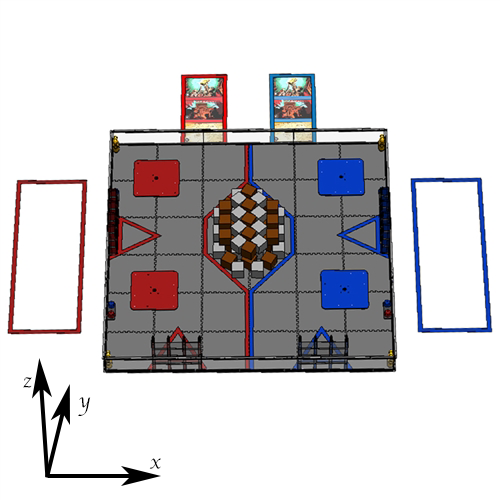
\includegraphics[width=10cm]{field_coordinate}
    
    $(0, 0, 0)$ is defined as the bottom left corner of the field.
    
    All units are assumed to be in meters (or preconverted).
\end{center}
\clearpage

The accelerometer gives us an acceleration vector $\vec{a}_{raw}$
where all units are in $m/s^2$. The gyroscope gives us the angular velocity vector
$\vec{\omega}_{raw}$, where the equivalent values of $x$, $y$, and $z$ in the vector denote the angular velocities in $rad/s$ around the respective axis. This image provides a better visualization of the concept:

\begin{center}
    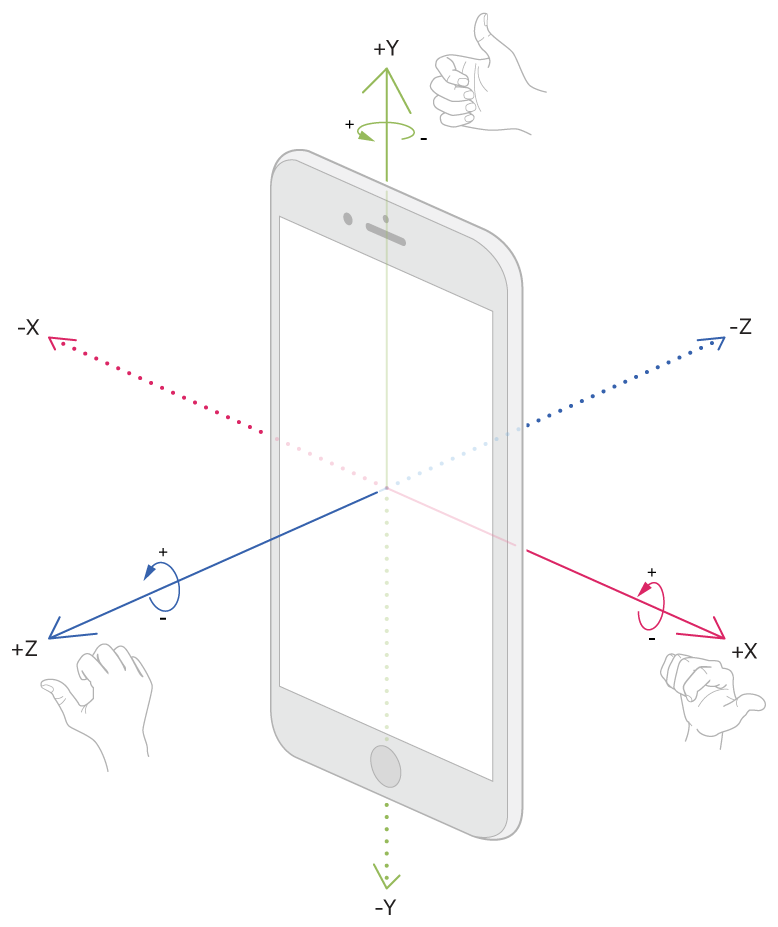
\includegraphics[width=6cm]{gyroscope_axes}
\end{center}

As one can see, a positive value for, say, $\omega_x$ means a counterclockwise value when looking down from the top of the $x$-axis. For those who are curious, this formalization is known as \href{https://en.wikipedia.org/wiki/Euler_angles#Tait\%E2\%80\%93Bryan_angles}{Tait-Bryan angles}. An easy way to find the direction of positive rotation around an axis is to use the right-hand rule, as shown in the image.

We generalize any angular vector conceptually as a counterclockwise rotation when viewed from the top of the vector, with an angular magnitude of the vector.
% include picture from wiki here - svg not supported, must be converted

We must also know the orientation of the phone on the robot and the positions of the image tracking targets on the field - this way we can get the actual orientation of the robot from the images. As you may know, there is a transformation matrix $T$ which will transform a column vector $\vec{a}$ by the given transformations, e.g. rotations or translations. This is simply done by multiplying:
\[
    \vec{a}_{transformed} = \vec{a}T
\]
Do note that order does matter in matrix transformation.


The Vuforia library provides us with methods to generate these transformation matrices with given values for rotation or translation. For example:
\clearpage
\begin{minted}{java}
// Creating a column vector with values x,y,z
OpenGLMatrix column_vector = OpenGLMatrix.translation(x, y, z);
// creating a matrix that rotates 90 degrees in x and -45 degrees in y
OpenGLMatrix rotation_matrix = Orientation.getRotationMatrix(
    AxesReference.EXTRINSIC, AxesOrder.XYZ,
    AngleUnit.DEGREES, 90, -45, 0);
// rotating the column vector by the rotation matrix
OpenGLMatrix transformed_vector = column_vector.multiplied(rotation_matrix);
// everything combined into one: creating a pose for a target
OpenGLMatrix phoneLocationOnRobot = OpenGLMatrix
    .translation(x, y, z)
    .multiplied(Orientation.getRotationMatrix(
        AxesReference.EXTRINSIC, AxesOrder.XYZ,
        AngleUnit.DEGREES, 90, -45, 0));
\end{minted}

\section{Physics knowledge}
% TODO: Add explanation for difference between dot and cross product
Some bits of knowledge to understand before beginning:
\begin{itemize}
    \item The relationship between the tangential velocity $\vec{v}$ of a particle moving in a circular path with a radius $r$ with an instantaneous angular velocity $\vec{\omega}$ is simply:
    \[
        |\vec{v}| = |r\vec{\omega}|
    \]
    This can easily be derived by the circumference equation of a circle. We know that:
    \[
        C = 2 \pi r
    \]
    Here, the $2\pi$ can be interpreted as the radian measure of the entire circle.
    Thus, if we only take a part of that radian measure, then we get the arc length of
    that part of the circle. This gives us:
    \[
        d = r \theta
    \]
    Dividing by time:
    \[
        \frac{d}{t} = r \frac{\theta}{t}
    \]
    \[
        v = r \omega
    \]
    We clearly see that these operations can easily be applied to vectors in the same way, as there is only scalar operations involved, giving us our original equation.
    % add an explanation for this later
    \item Velocity is the rate of change of position, and acceleration is the rate of change of velocity.
    In raw calculus terms:
    \[
        \vec{v} = \frac{d\vec{p}}{dt}
    \]
    \[
        \vec{a} = \frac{d\vec{v}}{dt}
    \]
    Inversely, we can also say that:
    \[
        \vec{p} = \int_{0}^{T} \vec{v} dt + \vec{C}
    \]
    \[
        \vec{v} = \int_{0}^{T} \vec{a} dt + \vec{C}
    \]
    where $\vec{C}$ is some constant vector.
    \item The cross product of two vectors $\vec{a}$ and $\vec{b}$ is the perpendicular
    to both vectors, and order matters. In addition:
    \[
        \vec{a} \times \vec{b} = |\vec{a}||\vec{b}| \sin \theta
    \]
    Where $\theta$ is the angle between the vectors. This can be visualized with the 
    right-hand rule:
    \begin{center}
        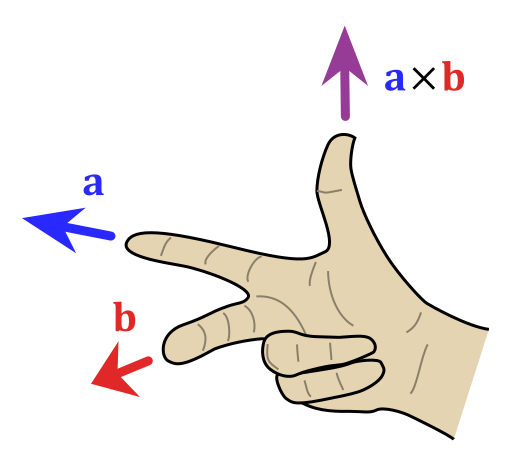
\includegraphics[width=6cm]{rh_rule}
    \end{center}
\end{itemize}

\section{Deriving the Transformation Matrix}

We have to acknowledge that the initial position of the phone is that it is centered at $(0, 0, 0)$ with the screen on the $+z$ axis, top edge of the phone on the $+y$ axis, and right edge of the phone on the $+x$ axis. An illustration is included below.

\section{Given Values}
\begin{itemize}
    \item The transformation matrix that transforms phone vectors into robot vectors, $\vec{M}$.
    \item The phone's position relative to the axial center of the robot, $\vec{p}$
    \item The phone's accelerometer values as a linear acceleration vector, $\vec{a}_{phone}$.
    \item The phone's gyroscope values as an angular velocity vector with magnitude in radians and in Tait-Bryan form, $\vec{\omega}_{phone}$.
    \item The initial position of the robot $\vec{c}$ at $t=0$.
    \item The change in time, $\Delta t$
    \item The time since the start, $T$
\end{itemize}

\section{Finding The Simple Change in Position}
We know that we can simply transform the phone acceleration with the given transformation matrix, giving us:
\[
    \vec{a}_{robotSimple} = \vec{a}_{phone} M
\]
In addition, we know that:
\[
    \vec{v} = \int_{0}^{T} \vec{a} dt
\]
Clearly:
\[
    \vec{v}_{robotSimple} = \int_{0}^{T} \vec{a}_{phone} M dt
\]
Using the fact that matrix multiplication is distributive and the idea of Riemann Sums,
\[
    \vec{v}_{robotSimple} = (\int_{0}^{T} \vec{a}_{phone} dt) M
\]

The naive thought is that we can simply integrate this velocity over time in order to get our final position with no other hassle, but this line of reasoning is incorrect. Because the phone itself is off-center relative to the axial center of the robot, we must account for the acceleration/velocity that the phone will give us even when the robot is rotating in place.
\clearpage
\section{Deriving Excess Velocity Due to Rotation}
We begin by considering an arbitrary particle at a position $\vec{r}$ that has an angular velocity $\vec{\omega}$ around $(0,0,0)$ and a tangential velocity $\vec{v}$. For simplicity, we consider each component of rotation separately. Here, the rotation around the z-axis is illustrated.
\begin{center}
    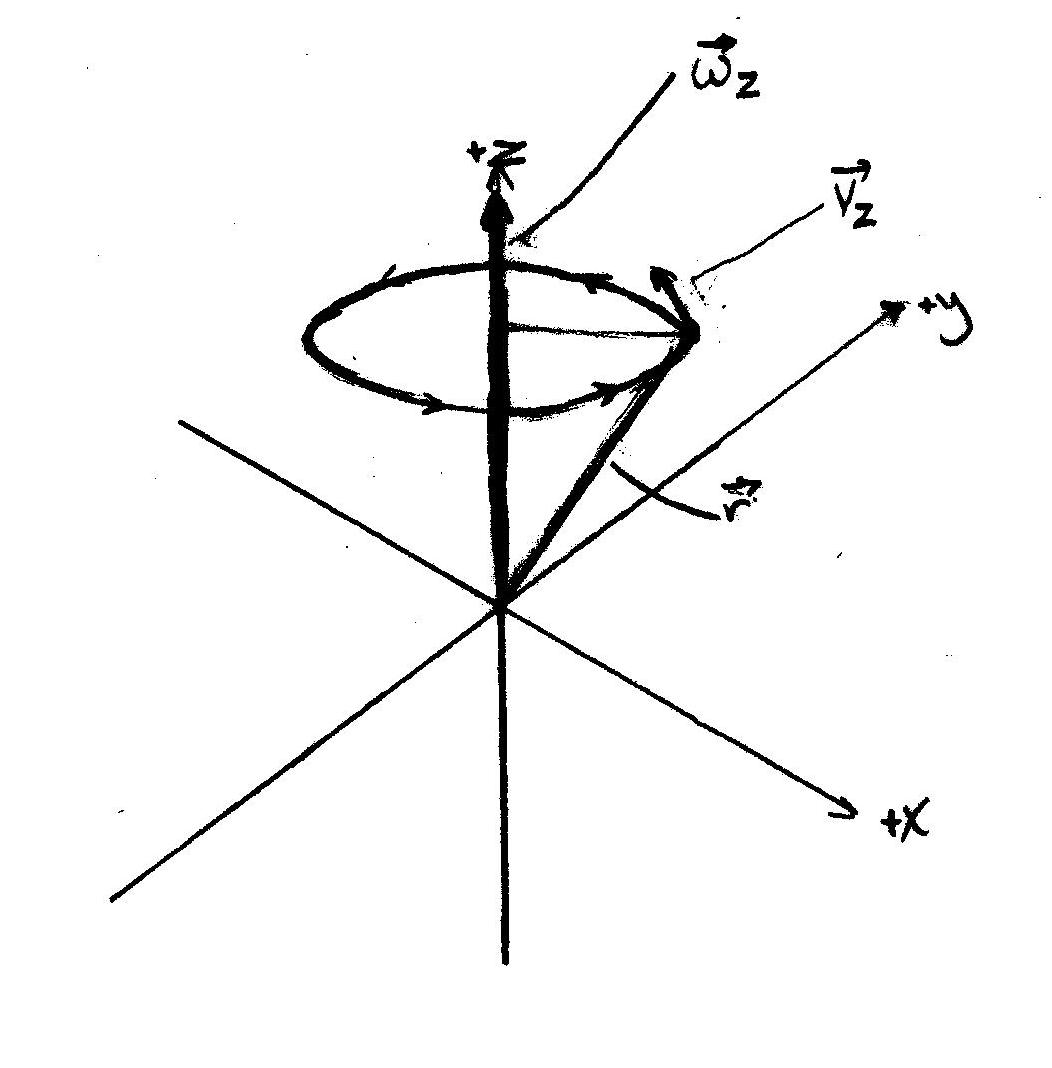
\includegraphics[width=6cm]{angular_1}
    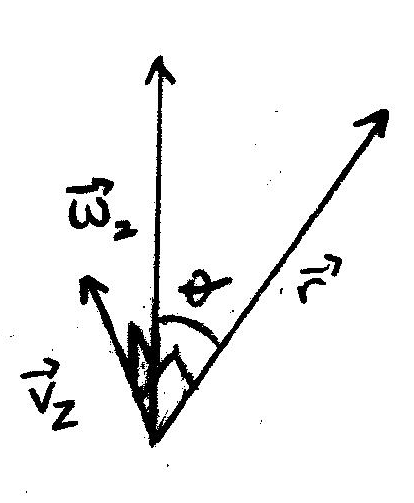
\includegraphics[width=6cm]{angular_2}
\end{center}

As one can clearly see from diagram 2, both $\vec{\omega}_z$ and $\vec{r}$ are perpendicular to $\vec{v}_z$. In addition, logically, as the angle between $\vec{\omega}_z$ and $\vec{r}$ increases, we know that $\vec{v}_z$ also increases. We also know that the cross product is defined as:
\[
    \vec{a} \times \vec{b} = |\vec{a}||\vec{b}|\sin \theta
\]
$\sin \theta$ is also positively correlated with $\theta$. We know that the further away something is from the center of rotation, the faster its tangential speed is, which implies that $|\vec{v}_z|$ is positively correlated with the product of $|\vec{\omega}|$ and $|\vec{r}$. This leads us to conclude that:
\[
    \vec{v}_z = \vec{\omega}_z \times \vec{r}
\]
We can do the same for all of the other axes, giving us
\[
    \vec{v}_x = \vec{\omega}_x \times \vec{r}
\]
\[
    \vec{v}_y = \vec{\omega}_y \times \vec{r}
\]
Clearly:
\[
    \vec{v} = \vec{v}_x + \vec{v}_y + \vec{v}_z
\]
Substituting:
\[
    \vec{v} = \vec{\omega}_x \times \vec{r} +
    \vec{\omega}_y \times \vec{r} +
    \vec{\omega}_z \times \vec{r}
\]
Knowing that the cross product is distributive over addition,
\[
    \vec{v} = (\vec{\omega}_x + \vec{\omega}_y + \vec{\omega}_z) \times \vec{r}
\]
Simplifying leads us to conclude:
\[
    \vec{v} = \vec{\omega} \times \vec{r}
\]

To apply this to the phone-robot system, we need to have the angular velocity of the phone relative to the robot. Because of how angular vectors are simply the perpendiculars to the direction of rotation and essentially the same as any usual vector, we can treat angular vectors the same way we do with normal vectors and transform them in the same way. Thus,
\[
    \vec{\omega}_{robot} = \vec{\omega}_{phone} M
\]
We also know that:
\[
    \vec{v}_{rotation} = \vec{\omega}_{robot} \times \vec{p}
\]
Substituting:
\[
    \vec{v}_{rotation} = \vec{\omega}_{phone} M \times \vec{p}
\]

\section{Finalizing the Equations}
Now that we have considered the rotation case, we can finalize our equations. With the rotation considered, our abstract equation is:
\[
    \vec{v}_{robot} = \vec{v}_{robotSimple} - \vec{v}_{rotation}
\]
Substituting in our derived equations from the previous sections:
\[
    \vec{v}_{robot} = (\int_{0}^{T} \vec{a}_{phone} dt) M -
    \vec{\omega}_{phone} M \times \vec{p}
\]
Rewriting:
\[
    \vec{v}_{robot} = (\int_{0}^{T} \vec{a}_{phone} dt) M -
    (\vec{\omega}_{phone} \times \vec{p}) M
\]
Factoring:
\[
    \vec{v}_{robot} = ((\int_{0}^{T} \vec{a}_{phone} dt) -
    (\vec{\omega}_{phone} \times \vec{p})) M
\]
Integrating for position:
\[
    \vec{x}_{robot} = \int_{0}^{T} \vec{v}_{robot} dt
\]
Finally, we see that with a given time change $\Delta t$, the following equations are true:
\[
    \Delta \vec{v}_{robot} = (
        \vec{a}_{phone} \Delta t -
        \vec{\omega}_{phone} \times \vec{p}
        ) M
\]
\[
    \Delta \vec{x}_{robot} = \vec{v}_{robot} \Delta t
\]
\clearpage
\section{Implementation in code}
We first implement the cross product for vectors since it is not provided. Implementation is based exactly off the wikipedia entry, and is not necessary to show. The method itself is implemented as a static method in the \verb|ExtendedMath| class. For the most part, assume it works.


\end{document}
